\documentclass[10pt]{standalone}
\usepackage[utf8]{inputenc}
\usepackage{pgf,tikz,pgfplots}
\pgfplotsset{compat=1.15}
\usepackage{mathrsfs}
\usetikzlibrary{arrows,patterns}
\pagestyle{empty}
\begin{document}

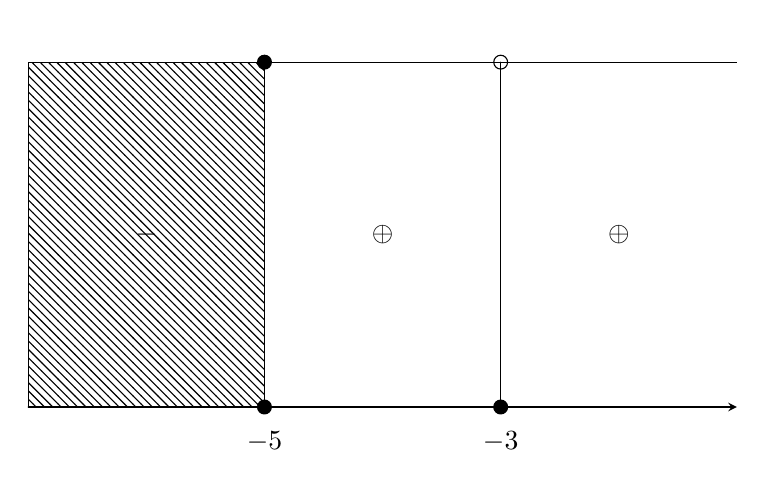
\begin{tikzpicture}[line cap=round,line join=round,>=triangle 45,x=1.0cm,y=1.0cm]
\begin{axis}[
x=1.0cm,%y=1.0cm,
axis x line=middle,
axis y line=none,
ticks=none,
xmin=-0.0,
xmax=9.0,
ymin=-0.2,
ymax=1.1,
]
\clip(-0.5,-0.2) rectangle (9.0,1.1);
\draw[pattern=north west lines] (0,0) rectangle (3,1.0);
%\draw  (6.,1.5)-- (9.0,1.5);
%\draw  [dash pattern=on 2pt off 2pt](0.,1.5)-- (6.,1.5);
\draw [dash pattern=on 2pt off 2pt] (0.,1.)-- (3.,1.);
\draw  (3.,1.)-- (9.,1.);
\draw  (3.,1.)-- (3.,0.);
\draw  (6.,1.0)-- (6.,0.);
\begin{scriptsize}
\draw [fill=black] (3.,0.) circle (2.5pt);
\draw (3.0,-0.1) node {$-5$};
\draw [fill=black] (6.,0.) circle (2.5pt);
\draw (6.0,-0.1) node {$-3$};
\draw  [fill=black](3.,1.) circle (2.5pt);
\draw  (6.,1.0) circle (2.5pt);
\draw (1.5,0.5) node {$-$};
\draw (4.5,0.5) node {$\oplus$};
\draw (7.5,0.5) node {$\oplus$};
\end{scriptsize}
\end{axis}
\end{tikzpicture}
\end{document}